\documentclass[tikz,border=10pt]{standalone}
\usepackage{tikz}
\usetikzlibrary{calc}

\begin{document}
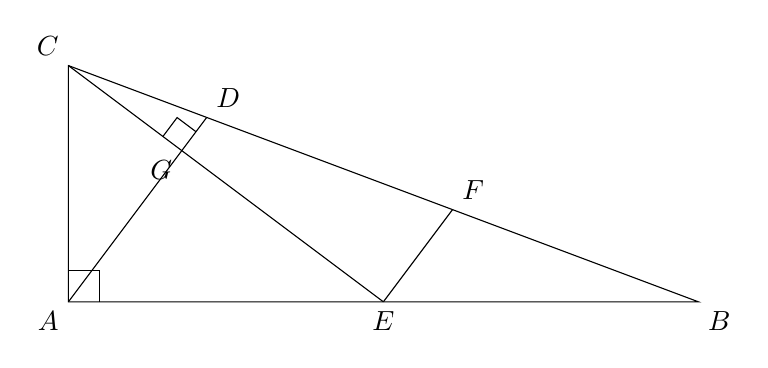
\begin{tikzpicture}
    % Define coordinates based on the analysis
    % A is origin (0,0)
    % B is on x-axis (8,0)
    % C is on y-axis (0,3)
    \coordinate (A) at (0, 0);
    \coordinate (B) at (8, 0);
    \coordinate (C) at (0, 3);
    
    % E is on AB. Placed at (4,0) to create the geometry.
    \coordinate (E) at (4, 0);
    
    % Line CE connects (0,3) and (4,0). Slope = -3/4.
    % Line AD is perpendicular to CE and passes through A(0,0). Slope = 4/3.
    % Equation of line AD: y = 4/3 x
    % Equation of line CB: y = -3/8 (x - 8)
    
    % Intersection D is where AD meets CB.
    % 4/3 x = -3/8 (x - 8) => 32x = -9x + 72 => 41x = 72 => x = 72/41
    \coordinate (D) at (72/41, 96/41);
    
    % Intersection G is where AD meets CE.
    % Equation of CE: y = -3/4 (x - 4)
    % 4/3 x = -3/4 x + 3 => 16x = -9x + 36 => 25x = 36 => x = 36/25
    \coordinate (G) at (36/25, 48/25);
    
    % Line EF is parallel to AD (slope 4/3) and passes through E(4,0).
    % Equation: y = 4/3 (x - 4)
    % Intersection F is where EF meets CB.
    % 4/3 (x - 4) = -3/8 (x - 8) => 32(x-4) = -9(x-8) => 32x - 128 = -9x + 72 => 41x = 200
    \coordinate (F) at (200/41, 48/41);
    
    % Draw the main triangle ABC
    \draw (A) -- (B) -- (C) -- cycle;
    
    % Draw the internal segments
    \draw (A) -- (D);
    \draw (C) -- (E);
    \draw (E) -- (F);
    
    % Draw right angle mark at A (between AC and AB)
    \draw (0, 0.4) -- (0.4, 0.4) -- (0.4, 0);
    
    % Draw right angle mark at G (between AD and CE)
    % We draw a small square corner.
    % Direction along GD (slope 4/3): (0.6, 0.8)
    % Direction along GC (slope -3/4, towards C): (-0.8, 0.6)
    % Scale factor for the mark size: 0.3
    \draw ($(G) + (0.18, 0.24)$) -- ($(G) + (-0.06, 0.42)$) -- ($(G) + (-0.24, 0.18)$);
    
    % Labels
    \node[below left] at (A) {$A$};
    \node[below right] at (B) {$B$};
    \node[above left] at (C) {$C$};
    \node[above right] at (D) {$D$};
    \node[below] at (E) {$E$};
    \node[above right] at (F) {$F$};
    \node[below left] at (G) {$G$};
\end{tikzpicture}
\end{document}
